\newpage
\section{Virtual Memory}

\label{sec:virt}
\subsection{Problem Space of Virtual Memory}
Virtual memory solves three problems \cite{virtualmemory2023}:
\begin{itemize}
    \item \textbf{Not enough memory, Memory fragmentation, and Security}
\end{itemize}
\begin{Def}[Not Enough Memory]

    Back then, computer memory was expensive, and many computers had very little memory (e.g., 4--1 GiB or even less).
    CPUs could only support up to 4 GiB of memory, as CPUs were 32-bit ($2^{32}$ addresses = $2^{32} bytes  = 4 GiB$). 
    On the other hand, 64-bit CPUs can support up to $2^{64}$ addresses = 16 million TB of memory.
\end{Def}

\begin{figure}[h]

    \hspace{-7em}
    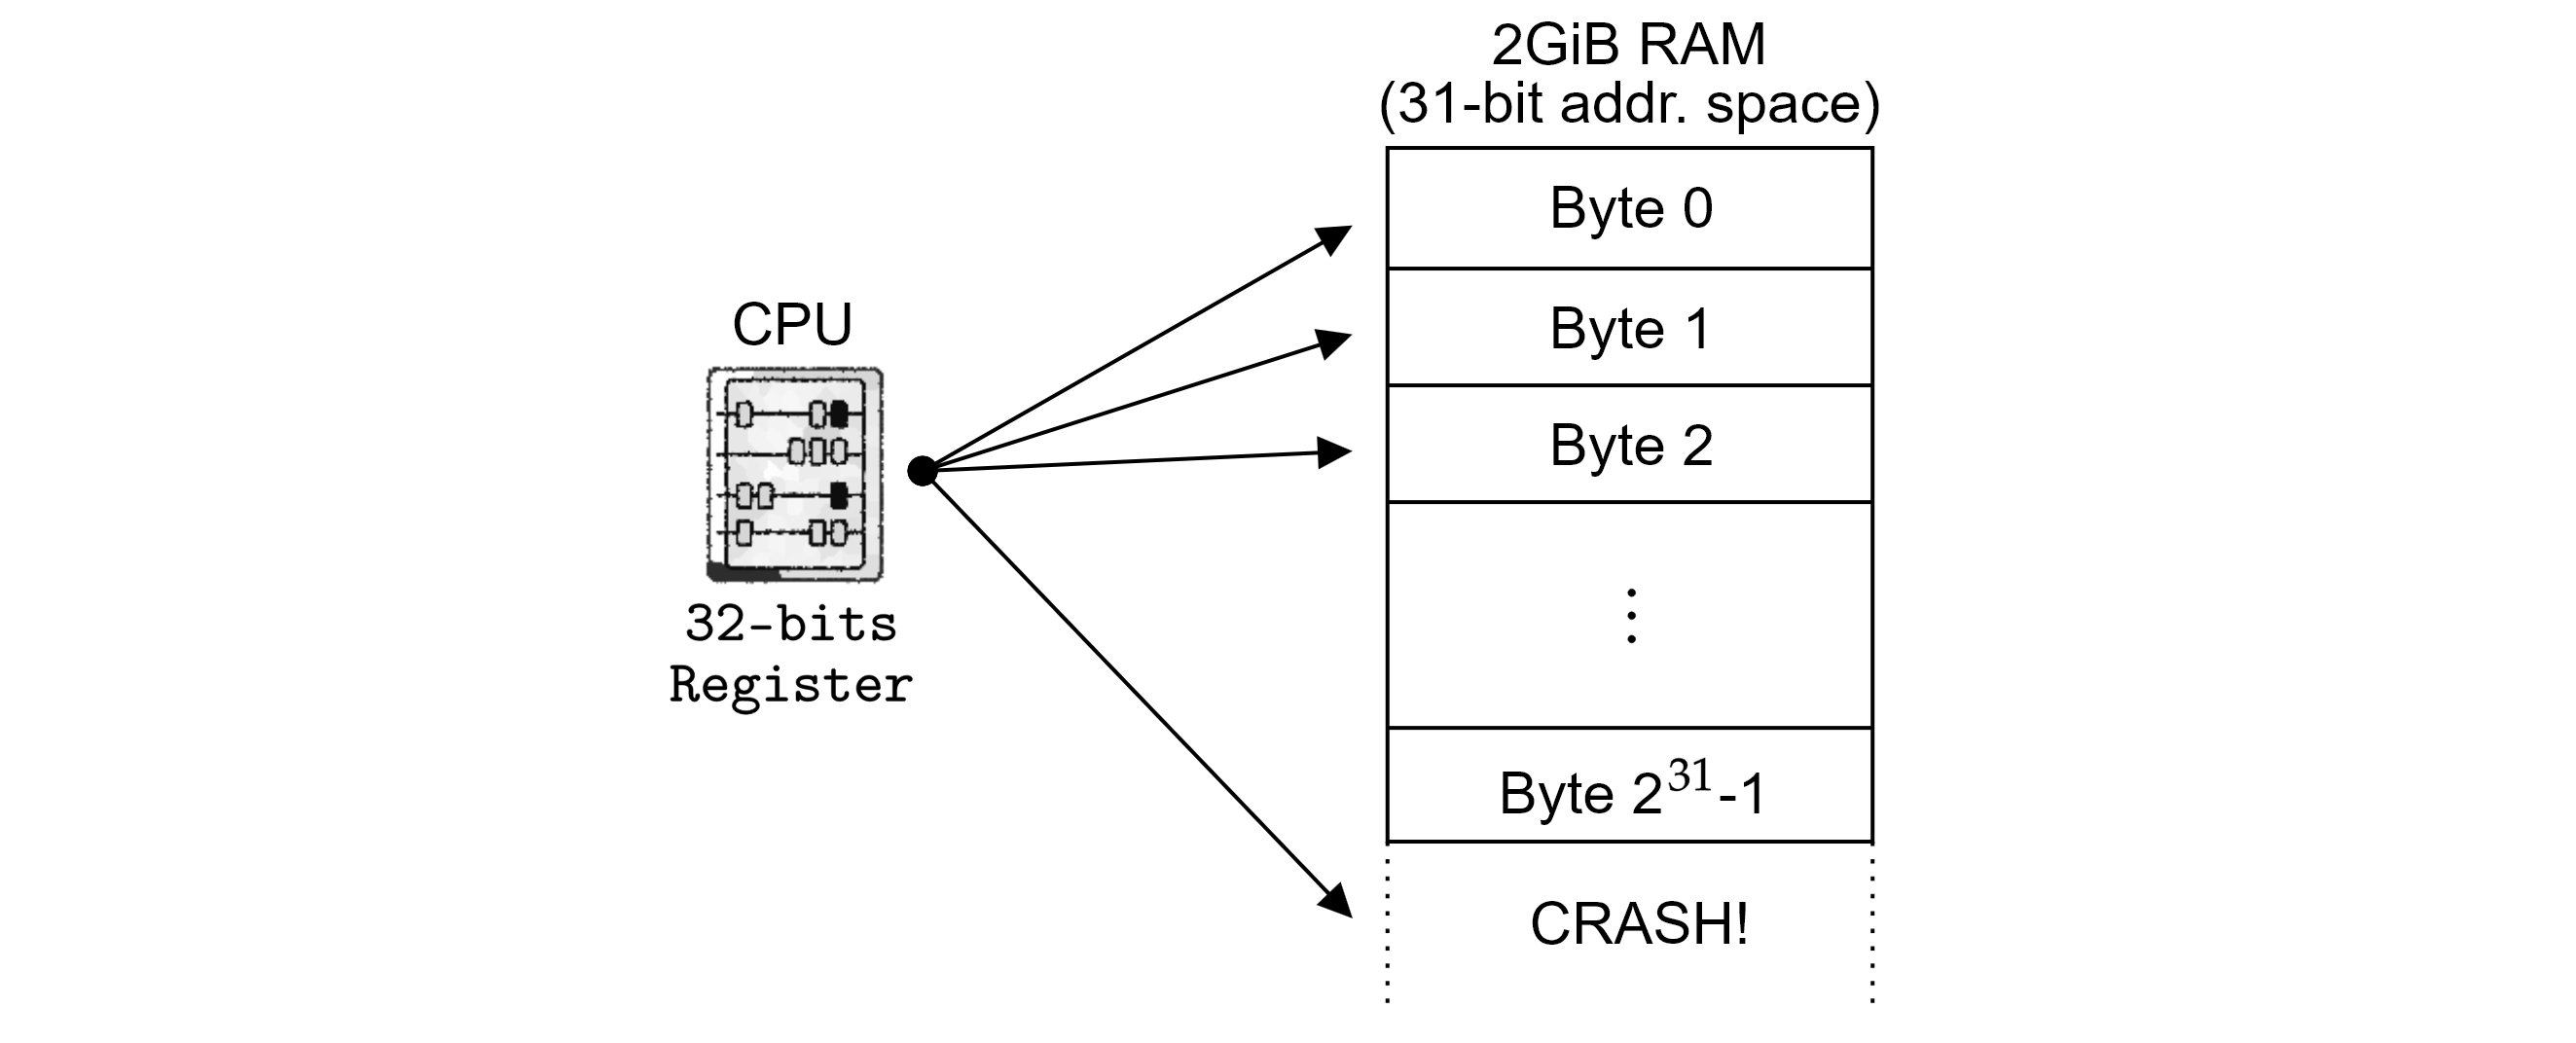
\includegraphics[width=1.3\textwidth]{Sections/virt/crash.png}
    
    \vspace{1em}
    \caption{A 32-bit CPU accessing 2 GiBs of RAM, where a crash happens when trying to access beyond the 31-bit address space.}
    
    \label{fig:virt1}
\end{figure}
\newpage 

\noindent
The next problem deals with multiple processes allocating and deallocating memory:

\begin{Def}[Memory Fragmentation]
    
    Memory can be thought of as a big array, where each cell is a resource a program can use.
    We want memory usage to be contiguous (i.e., no gaps or holes). So say we have an array 
    $$[O, O, O, O]$$

    \noindent
    Where $O$ represents free space in our array, each cell 1 GiB of space. If we have processes $A$ and $B$ take 1 and 2 GiBs respectively, we might have a memory layout of:
    $$[A, B, B, O,]$$

    \noindent
    If we then free process $A$, we might have a memory layout of:
    $$[O, B, B, O]$$
    \noindent
    Now, if another process $C$ needs 2 GiBs of memory, it will not be able to find a contiguous space of 2 GiBs, even though we have 2 GiBs of free space.
    This is called \textbf{memory fragmentation}.
\end{Def}

\noindent
Now finally we have the problem of protecting memory from other processes:

\begin{Def}[Memory Security]

    In a multi-process system, processes may have collisions when trying to access the same memory space.
    For example, if process $A$ is a weather service and process $B$ is some finance service, we don't want 
    the weather service to overwrite the same memory space where the finance service is storing critical data.
    This is called \textbf{memory security}.
\end{Def}

\noindent
So in theory we want to give each process it s own portion of memory, to solve overlapping access:
\begin{Def}[Virtual Memory]

    To solve process memory collisions, we give each process its own fictional view of memory, called \textbf{virtual memory}.
    Though for this to work, each virtual view is mapped to an actual place in the original memory we call \textbf{physical memory}.\\

    \noindent
    \textbf{Virtual and physical addresses} are the cells spaces themselves.
\end{Def}

\newpage 

\noindent
Consider the figure below showing how virtual memory works in theory:

\begin{figure}[h]
    \centering
    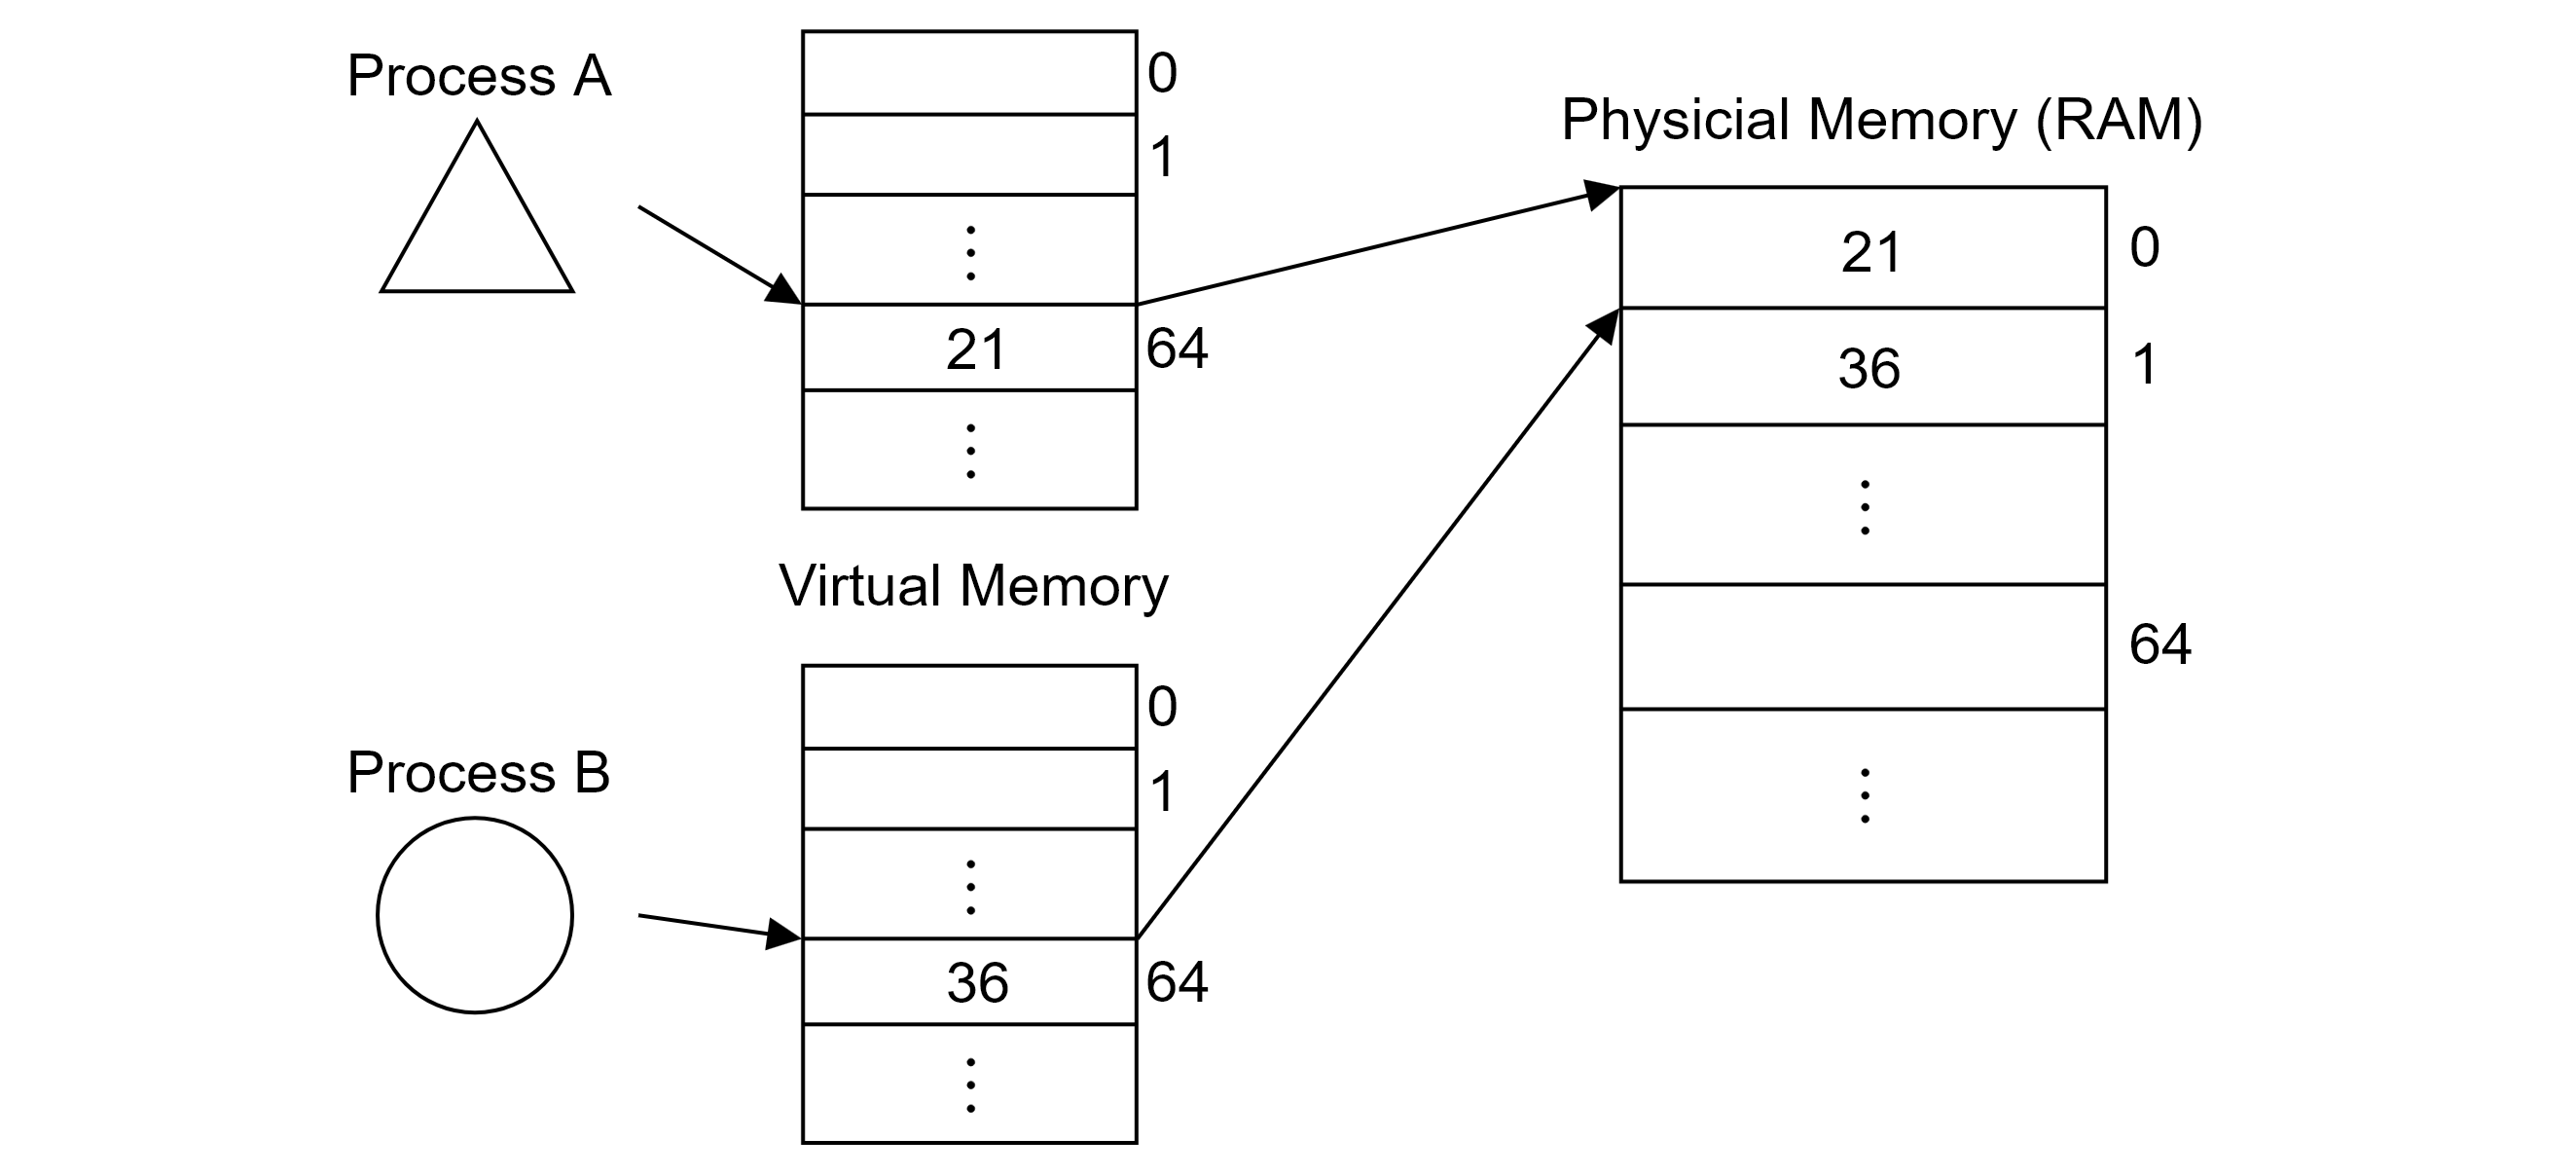
\includegraphics[width=\textwidth]{Sections/virt/virt.png}
    
    \vspace{1em}
    \caption{Processes $A$ and $B$ write to memory cell $64$ in their view of memory, but in reality they map 
    to different physical memory cells (0 and 1 respectively).}
    
    \label{fig:virt2}
\end{figure}

\noindent
A quick aside:

\begin{theo}[Physical Memory the CPU Accesses]

    In reality the CPU can access the physical memory of many other devices (e.g., hard drives, SSDs, etc.). In 
    addition, the OS takes up some of the physical memory as well. The rest is left to programs to use. The 
    program allocated space is the memory we refer to going forward as the \textbf{physical memory}.
\end{theo}

\noindent
Virtual memory solves the three problems we mentioned before:
\begin{Def}[Virtual Memory \& Not Enough Memory (Swapping)]

    The physical memory can be much smaller than what a program thinks it has in virtual memory. When a program tries to access memory 
    it does not have, the OS will \textbf{swap} physical memory to external storage to free up space. This means, while a program is not using 
    a portion of memory at a given time, the OS can swap it in and out depending on system needs.\\

    \noindent
    Memory that is swapped out is called \textbf{swap-memory}. Every time a we try to access such absent memory 
    in our mappings, it's called a \textbf{page fault} (more on this later).
\end{Def}

\newpage
\begin{Def}[Virtual Memory \& Fragmentation]

    Virtual memory allows programs to think they have contiguous memory. This simplifies their 
    memory management, while in reality the OS manages the split memory mappings.
\end{Def}

\begin{figure}[h]
    \centering
    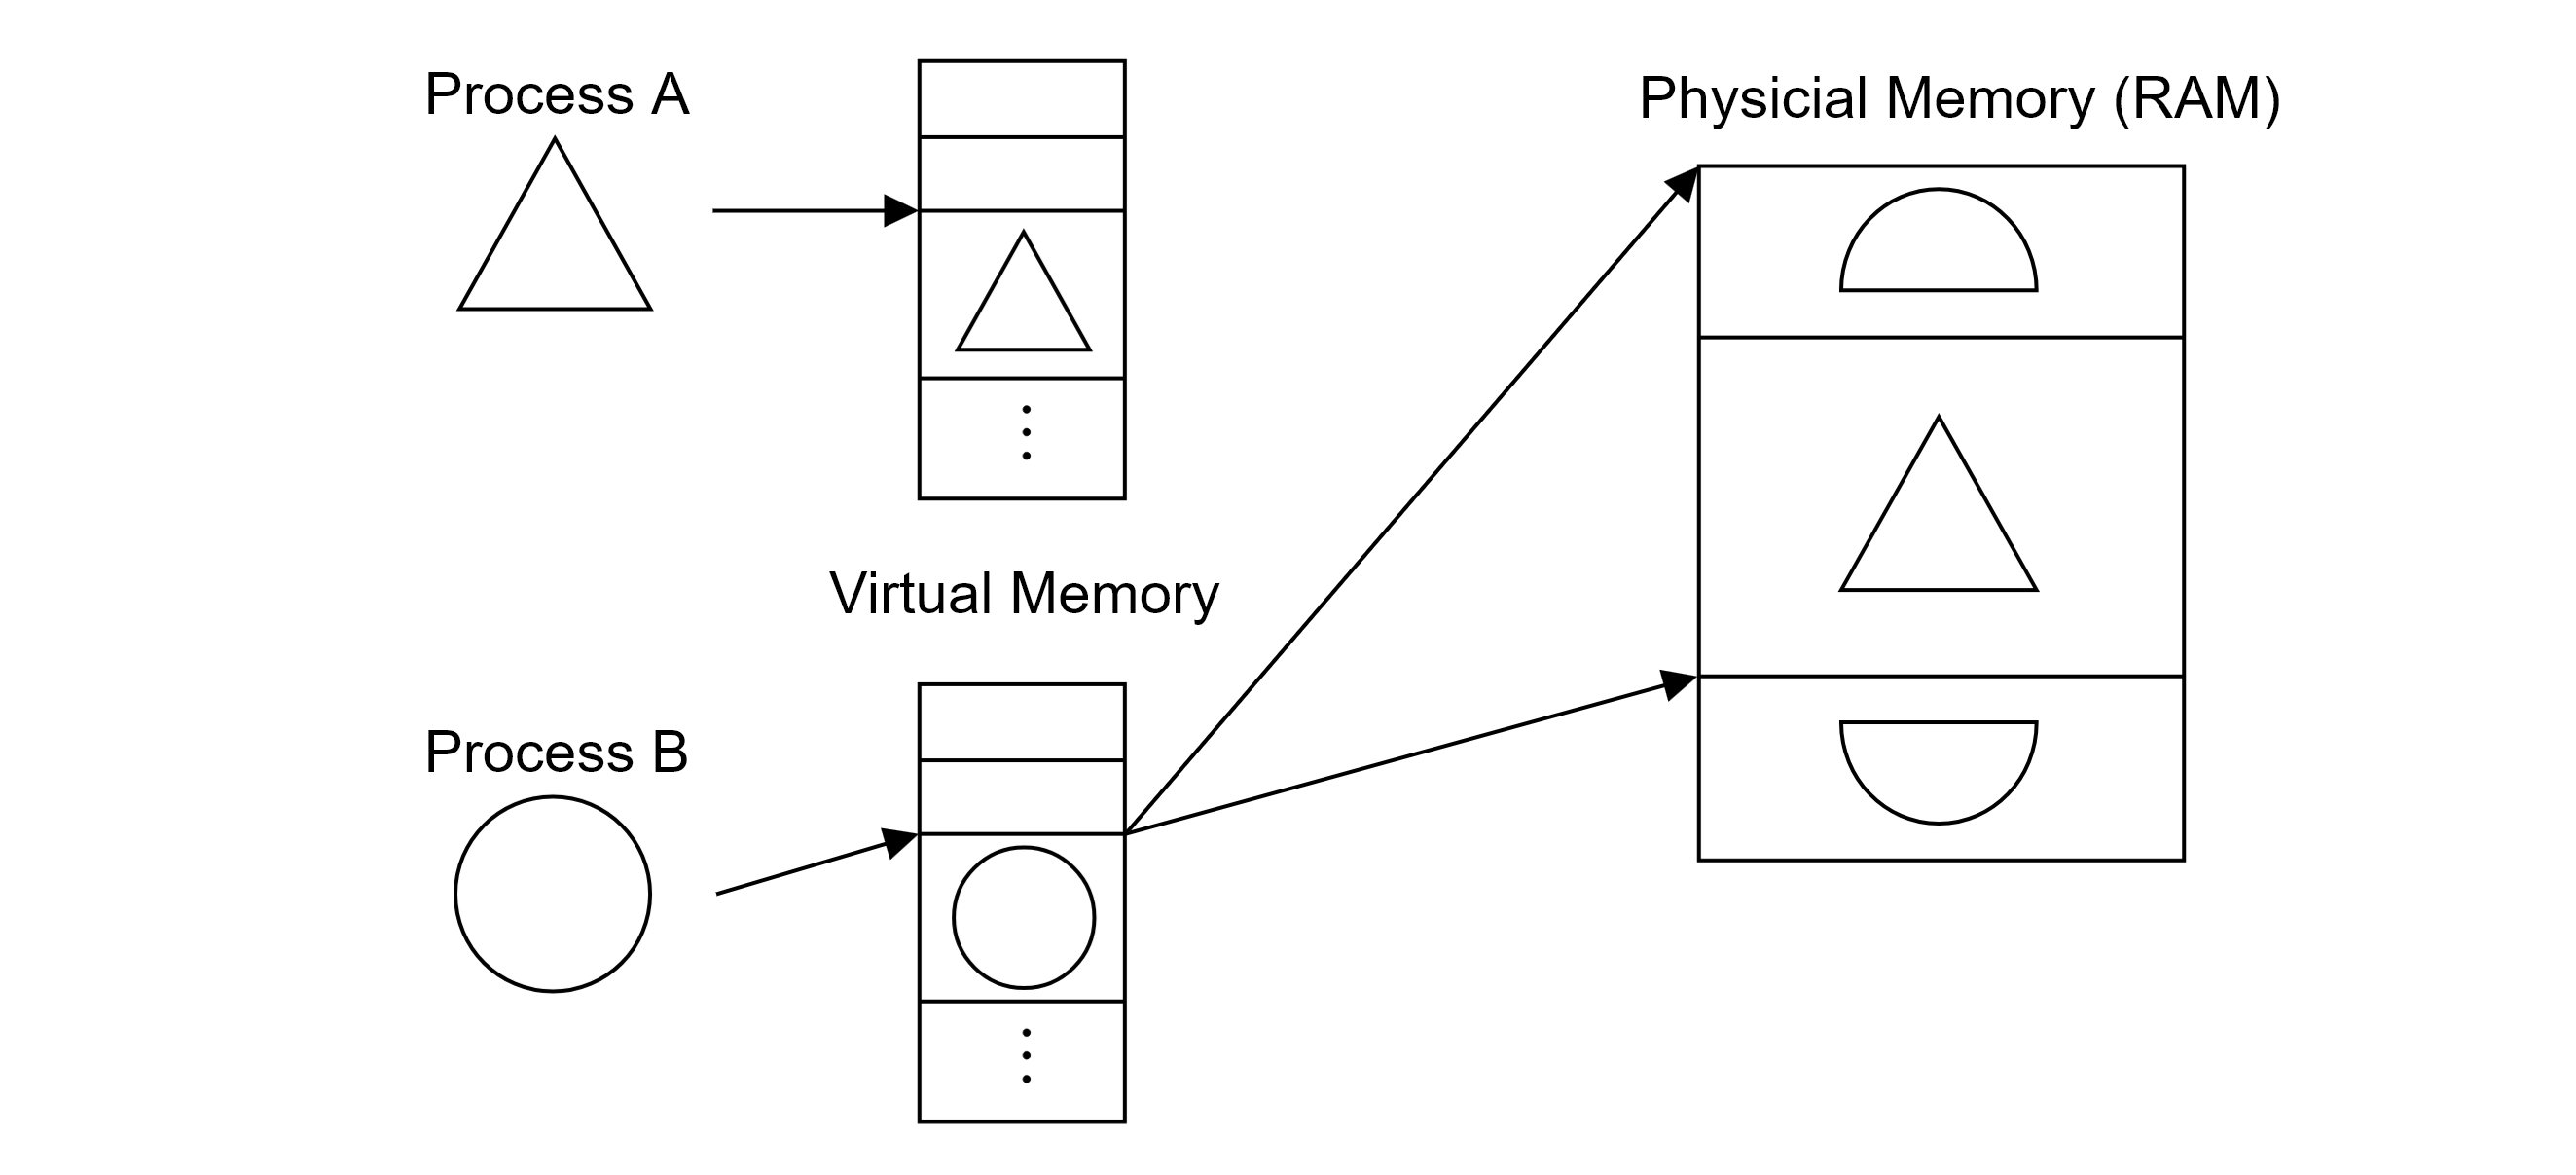
\includegraphics[width=\textwidth]{Sections/virt/frag.png}
    
    \vspace{1em}
    \caption{Here two processes $A$ and $B$ are using the same physical memory space. Both think they have 
    contiguous memory, but in reality, $B$ is split into two parts in the physical memory.}
    
    \label{fig:virt3}
\end{figure}

\begin{Def}[Virtual Memory \& Security]

    Memory cells are collision safe as memory mappings are not shared in physical memory; However, this would be 
    inefficient if say $A$ and $B$ depend on a secondary process $C$. In this case, $A$ and $B$ may share the same mapping to $C$'s memory.
\end{Def}

\subsection{Virtual Memory Implementation (Page Tables)}
\noindent
We discuss the mapping mechanism further in linking virtual to physical memory.
\begin{Def}[Page Tables]

    The OS keeps a \textbf{page table}, where each entry is a mapping of a virtual memory cell to a physical one, called a \textbf{Page Table Entry (PTE)}.
    CPUs work with words (32 bits = 4 bytes), so the page table has one entry for every word (address) in the virtual memory space.
\end{Def}

\newpage 

\noindent
We make the following observation:
\begin{theo}[Theoretical Page Table Space Complexity]

    If our CPU 32-bits, then there are $2^{32}$ addresses. CPUs speak in words, hence we'd need $2^{30}$ words, and thus $\approx$ 1 billion PTEs (4 GiB per table).
    This is too much memory to practically implement for each process.
\end{theo}

\noindent
We solve the above problem, via the following strategy:

\begin{Def}[Memory Chunking (Pages)]
    
    Instead of mapping each address to a PTE---which would be too large. We
    chunk the memory into \textbf{pages} reducing the number of PTEs needed. Typically, page sizes 
    are some power of 2, most commonly 4 KiB (4096 bytes), meaning 1024 words per page. This reduces our 
    page table requirement from 4 GiB to 4 MiB (1 Million PTEs). Despite moving 4 KiBs of data at a time, this works
    well in practice, as adjacent memory is often accessed together. 
\end{Def}

\begin{figure}[h]
    \centering
    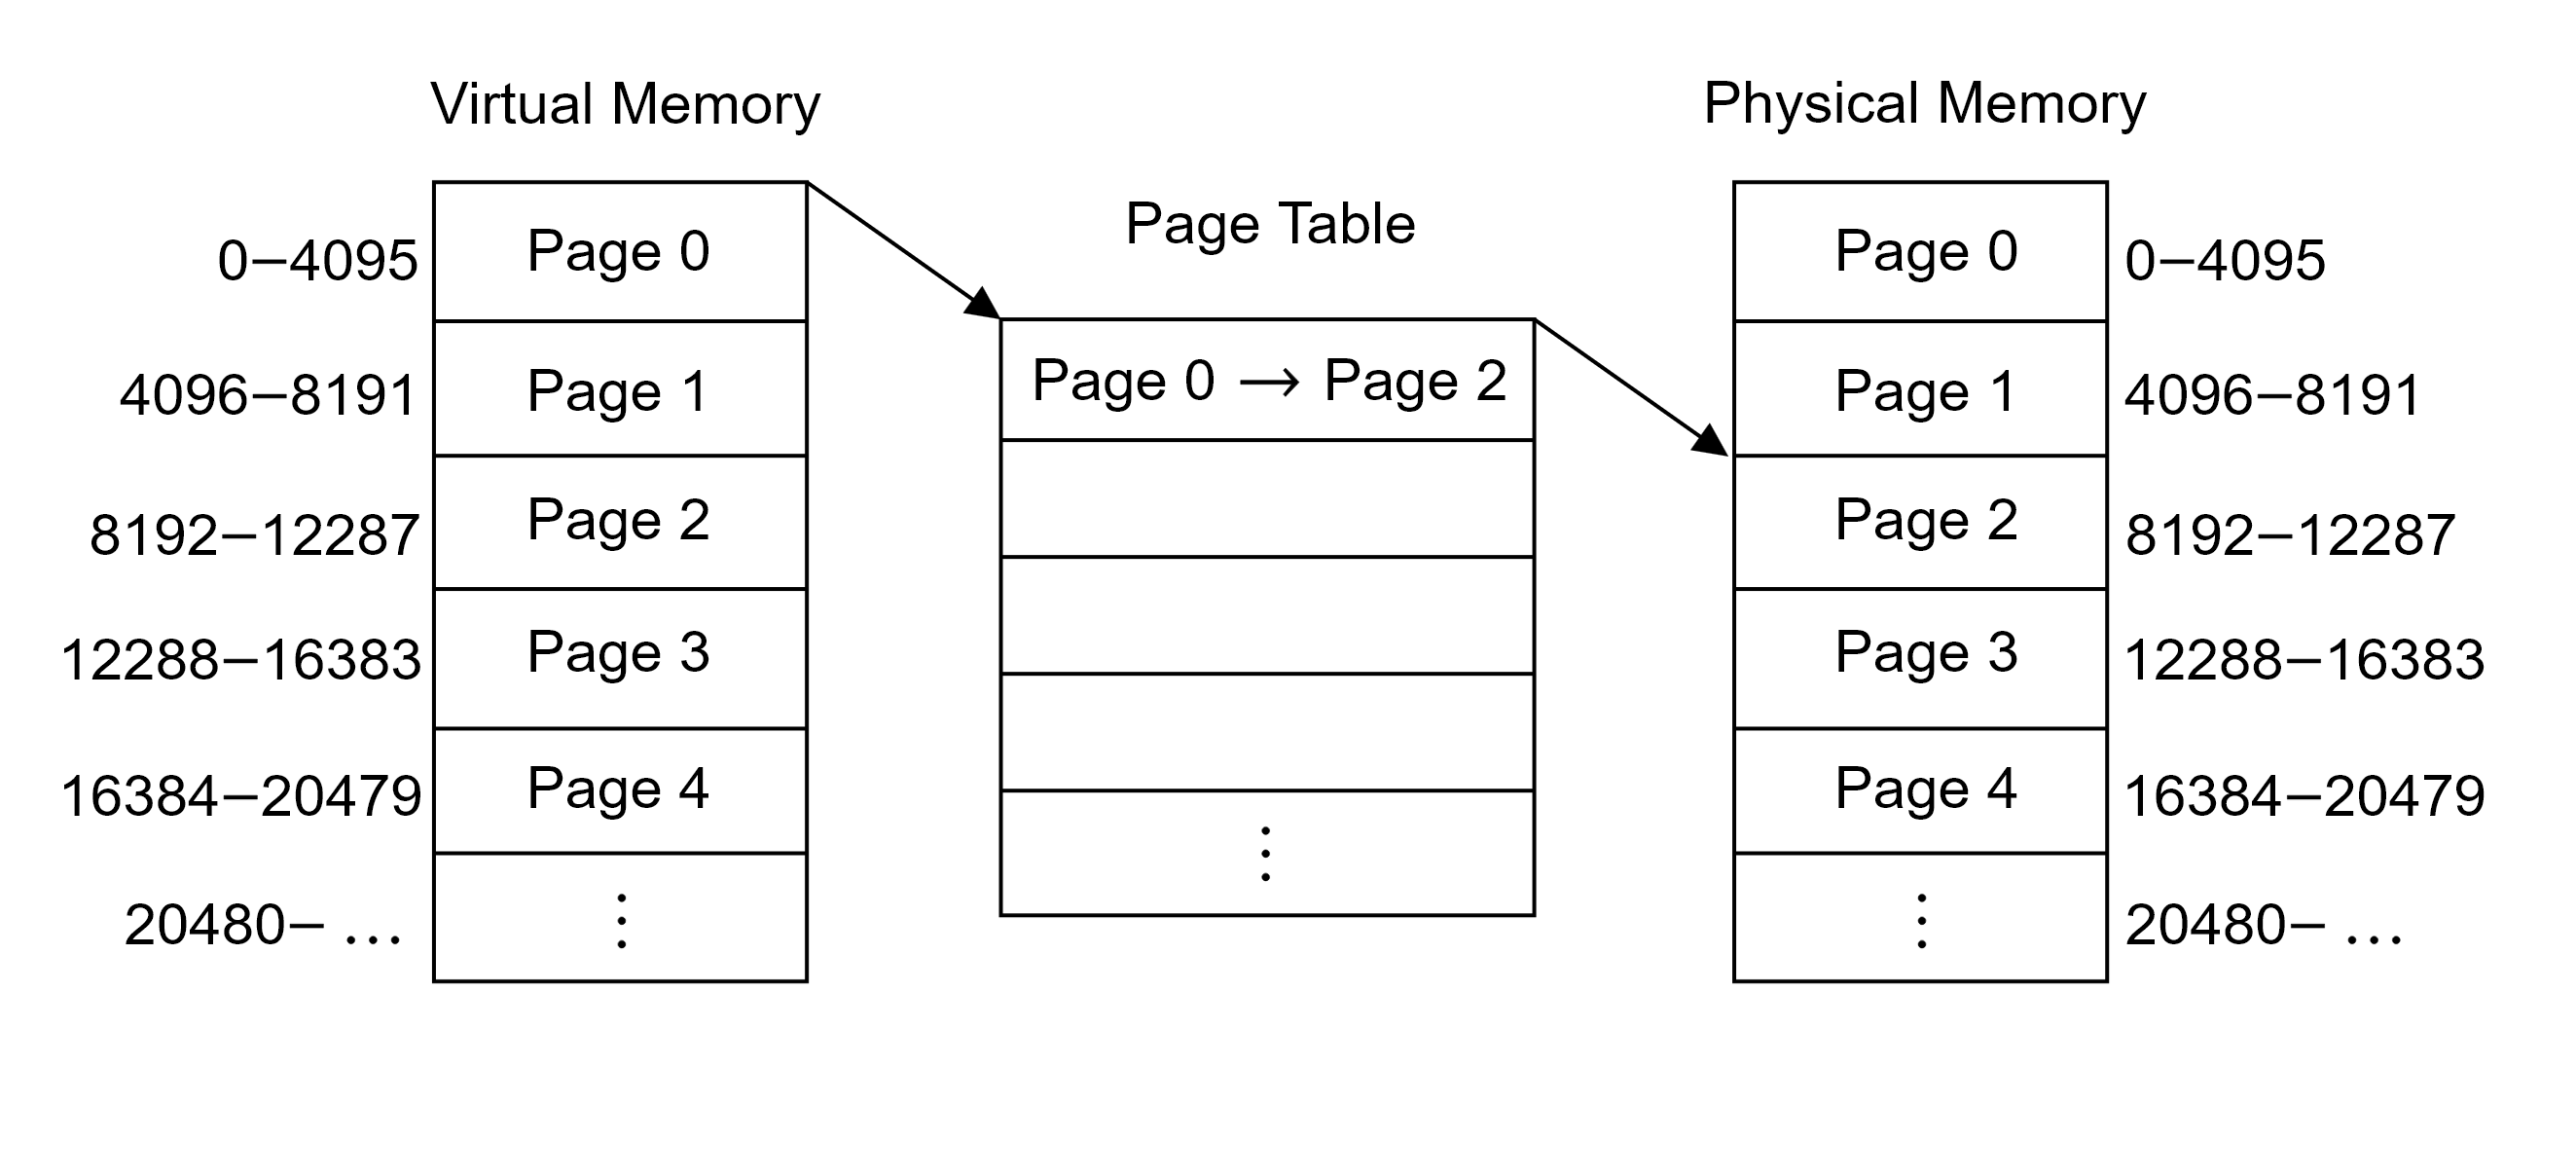
\includegraphics[width=\textwidth]{Sections/virt/page.png}
    
    \vspace{1em}
    \caption{A 4 MiB page table, each PTE 4 KiB (4096 bytes, 1024 words), showing mappings.}
    
    \label{fig:virt4}
\end{figure}


\noindent
One must ask themselves:
\begin{itemize}
    \item What is the relationship of how the Page Numbers are separated.
    \item Can we determine the page number given a specific address?
    \item How might we convert a virtual to a physical address given some address?
\end{itemize}
\noindent
We discuss the following on the next page.

\newpage 
\begin{Example}[Converting Virtual to Physical Memory (intuition)]

    \label{theo:virt2phys}
    We may find conversions from virtual to physical memory via the following formula: $$\text{PA} = \underbracket{(\text{VA}\ \%\ \text{Page Size})}_{\text{offset}} + \underbracket{(\text{Page Size} \cdot \text{Physical Page Number})}_{\text{Physical Page starting index}}$$
    \noindent
    Where $\%$ is modulo and Page Number = $\left\lfloor \frac{\text{Addr.}}{\text{Page Size}} \right\rfloor$. \textbf{However,} this is not the most efficient way,
    and is \underline{strictly for educational/intuition building} purposes.\\

    \noindent
    \rule{\textwidth}{0.4pt}\\

    \noindent
    Given the Figure (\ref{fig:virt4}), $104\to 8296$ from $104 + 4096 * 2 = 8296$.
\end{Example}
\begin{theo}[Converting Virtual to Physical Memory]

    Addresses are binary numbers, typically represents as hexadecimal (base 16) numbers.


    The first 12 bits of an address is the \textbf{offset}. The remaining higher-order bits yields the \textbf{page number}. To find the physical address, take the last 12 bits of the address, index the higher-order bits into the page table, and append the offset to the physical page number.
\end{theo}

\begin{figure}[h]
    \centering
    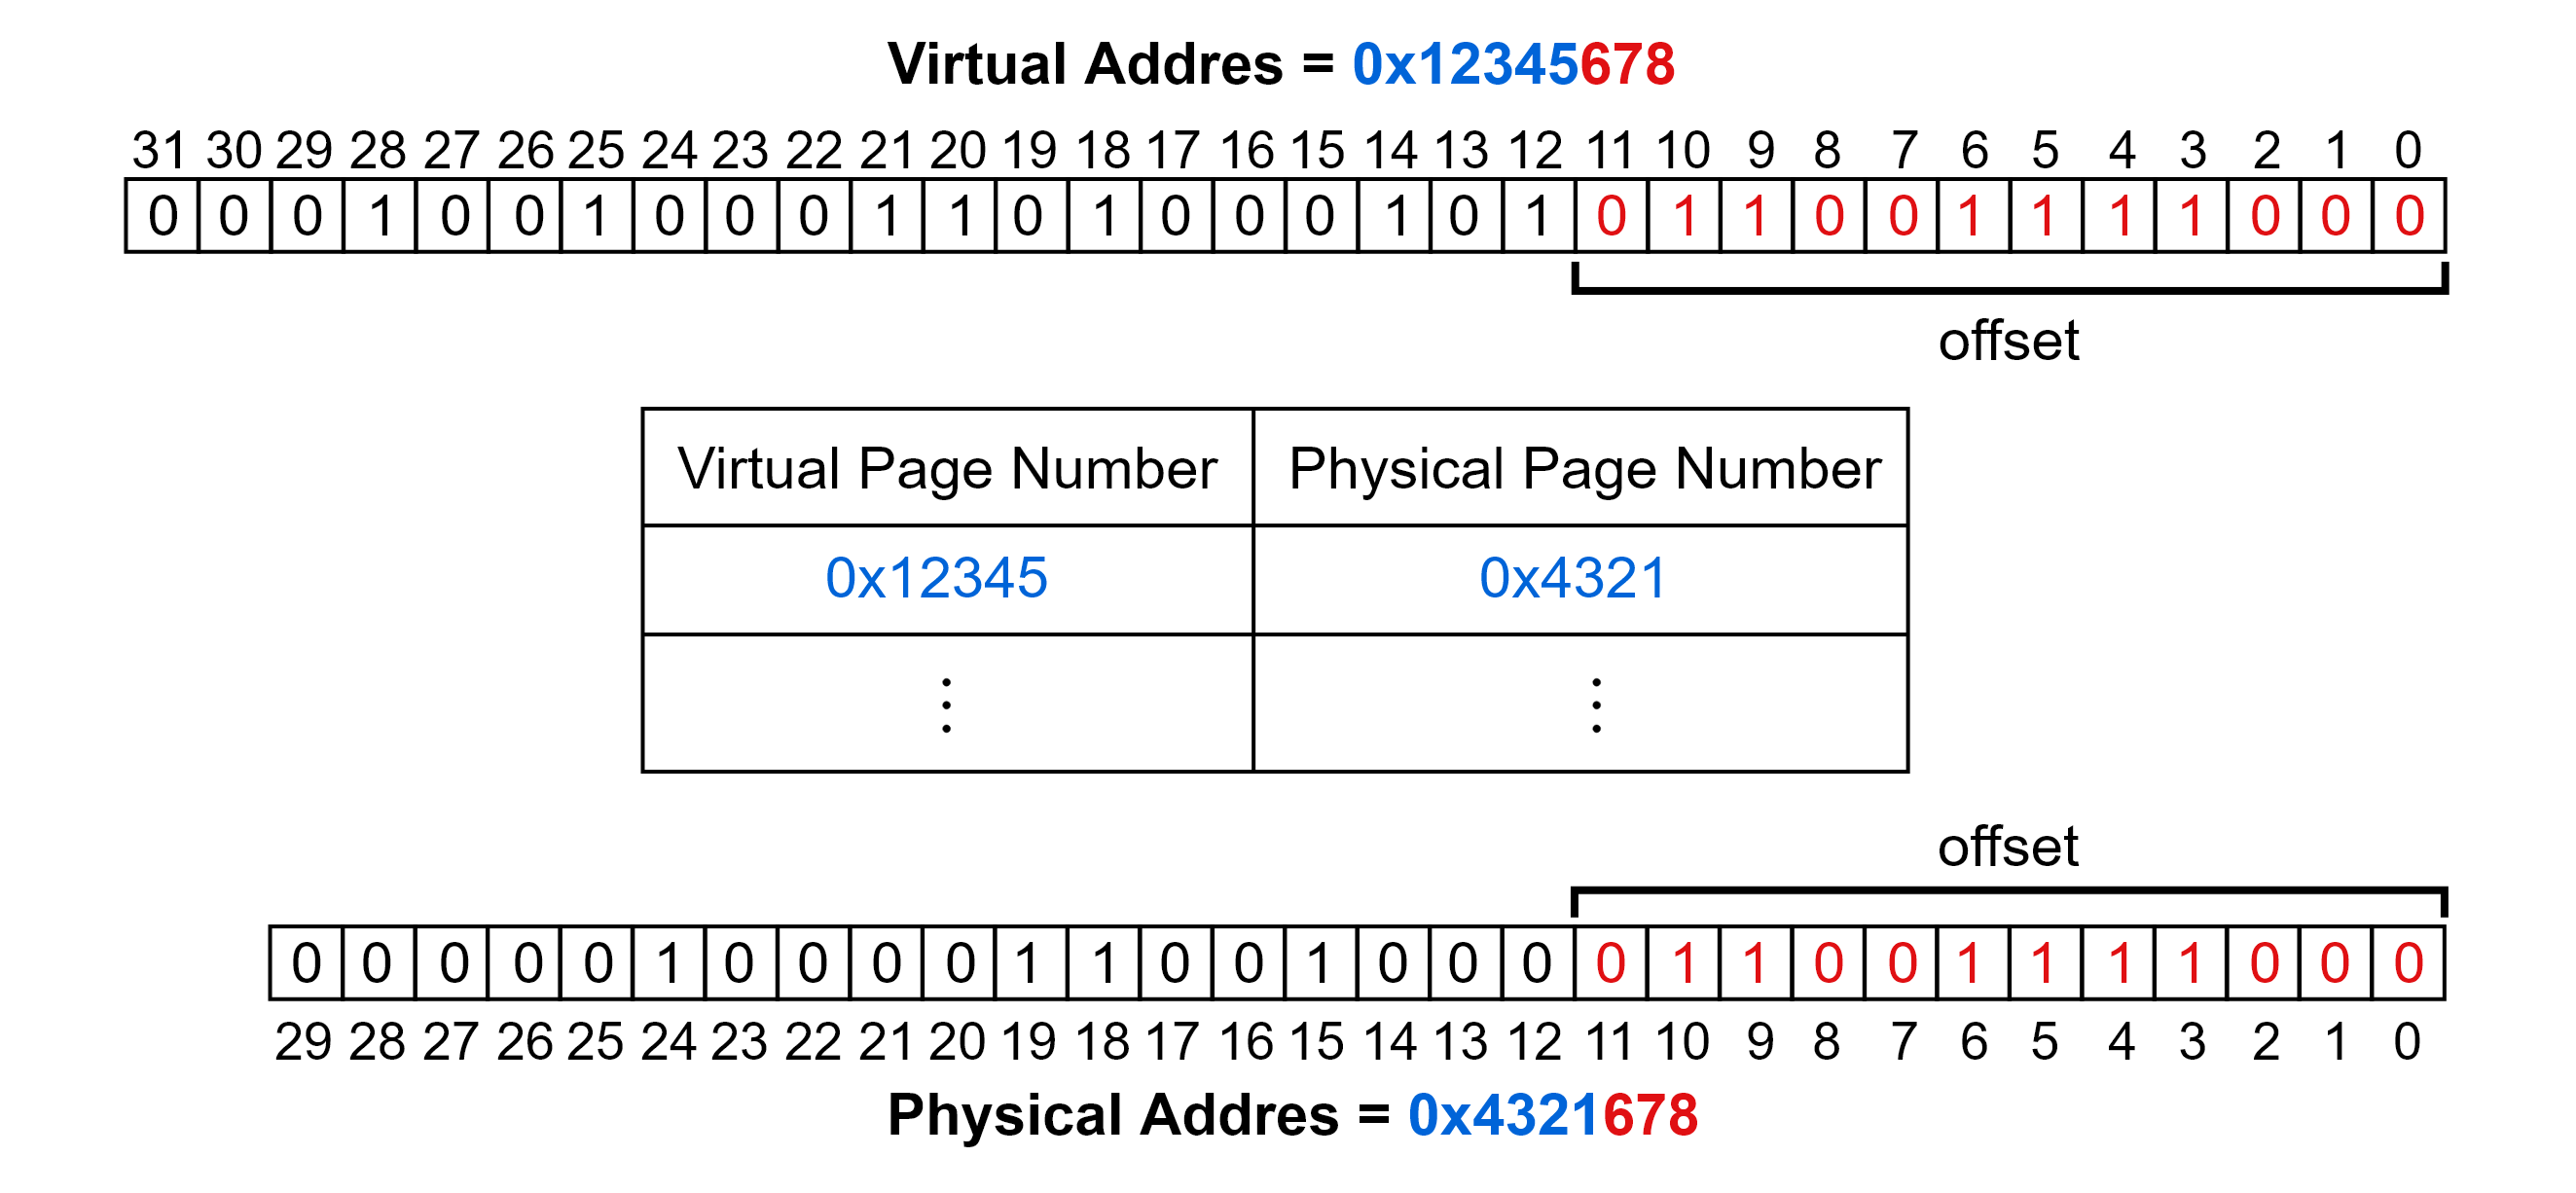
\includegraphics[width=\textwidth]{Sections/virt/conv.png}
    
    \vspace{1em}
    \caption{The conversion of 0x123456 (32-bit, 4 GiB) $\to$ 0x4321678 (30-bit, 1 GiB). Recall that if a accessing a page that is not in memory, causes a page fault, from which the OS with begin to swap memory with external storage devices.}
    
    \label{fig:virt5}
\end{figure}

\newpage 

\subsection{Page Faults \& Translation Lookaside Buffer (TLB)}

So far we have discussed how the mapping system of virtual memory works, but now we pivot to how the OS handles swapping data in and out of memory on page faults.

\begin{Def}[Swapping on Page Faults]

    A \textbf{page fault} occurs when a program tries to access a page that does not have a mapping in the page table. 
    The OS then picks the \textbf{least recently used (LRU)} page in the page table, and swaps it out to external storage. A page is \textbf{dirty} if it has been written to. In 
    such case, we write back its contents to external storage before swapping. If the page is not dirty, we may discard it on swap.
\end{Def}

\vspace{-1em}
\begin{figure}[h]
    \centering
    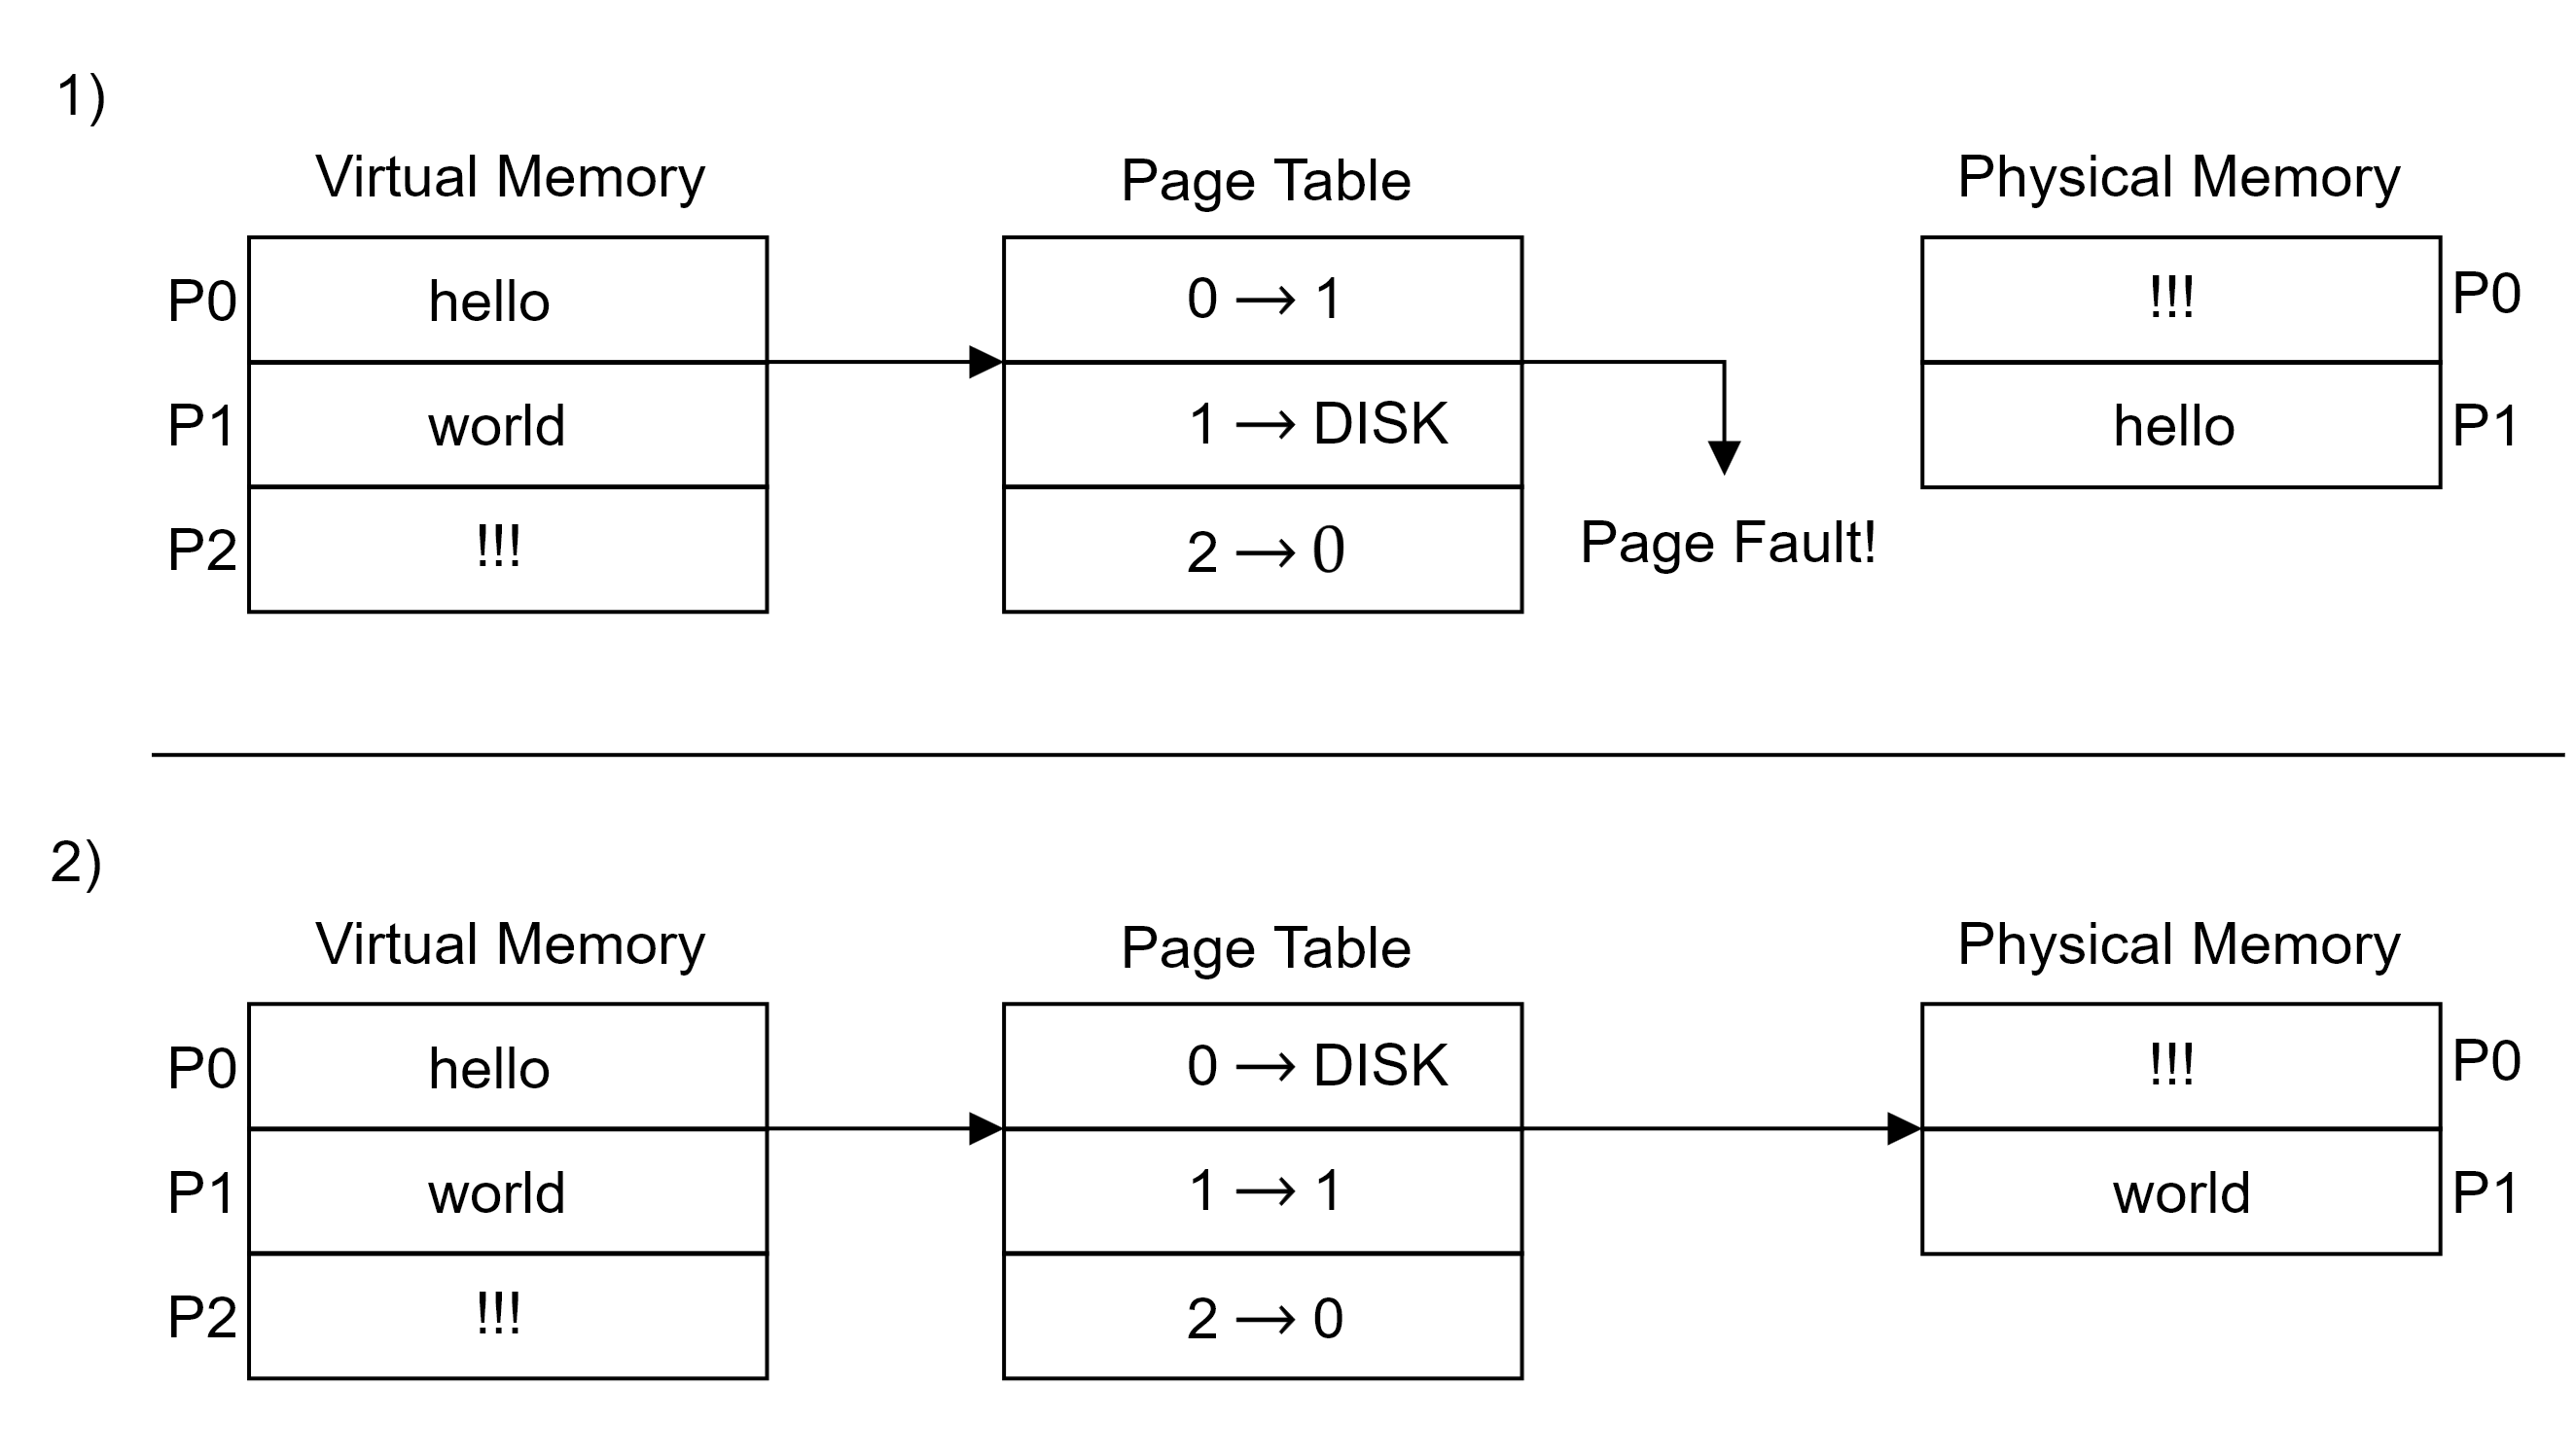
\includegraphics[width=\textwidth]{Sections/virt/pagefault.png}
    
    \vspace{1em}
    \caption{
        1) A page fault occurs when trying to access page 1. 2) The OS has swapped out page 0 to external storage (DISK), and now page 1 can be accessed.
        Note: This diagram is for illustrative purposes, virtual memory does not contain data, only addresses binding to physical memory.
        }

    \label{fig:virt6}
\end{figure}

\begin{Def}[Direct Memory Access (DMA)]

    Page faults are expensive, as swapping data with I/O devices may take some time. Modern CPUs have a \textbf{Direct Memory Access (DMA)} module, which allows I/O devices to access memory directly, while the CPU completes other tasks. 
\end{Def}

\noindent
Still our routine of mapping is expensive in it of itself.
\begin{Def}[Translation Lookaside Buffer (TLB)]

    The mapping process includes three steps:
    \begin{enumerate}
        \item Index the page table: Access Memory (RAM).
        \item Convert Addresses: Computation.
        \item Interact: Access Memory (RAM).
    \end{enumerate}
    \noindent
    To speed this up, we create a small cache of the most recent Page Table Lookups, called the \textbf{Translation Lookaside Buffer (TLB)}. If a 
    page in not in the TLB, we must preform the translation then load it into the TLB for future use.\\

    \noindent
    Every successful TLB lookup is called a \textbf{hit}, while a failed lookup is called a \textbf{miss}. The \textbf{hit time} and \textbf{miss time} are the time it takes to access the TLB and page table respectively (measured in CPU clock cycles).
    The \textbf{hit rate} is the ratio of hits to the total number of lookups.\\

    \noindent
    Modern CPU architectures usually have two TLBs, one for instructions (\textbf{ITLB}) and one for data (\textbf{DTLB}).
\end{Def}

\begin{figure}[h]
    \centering
    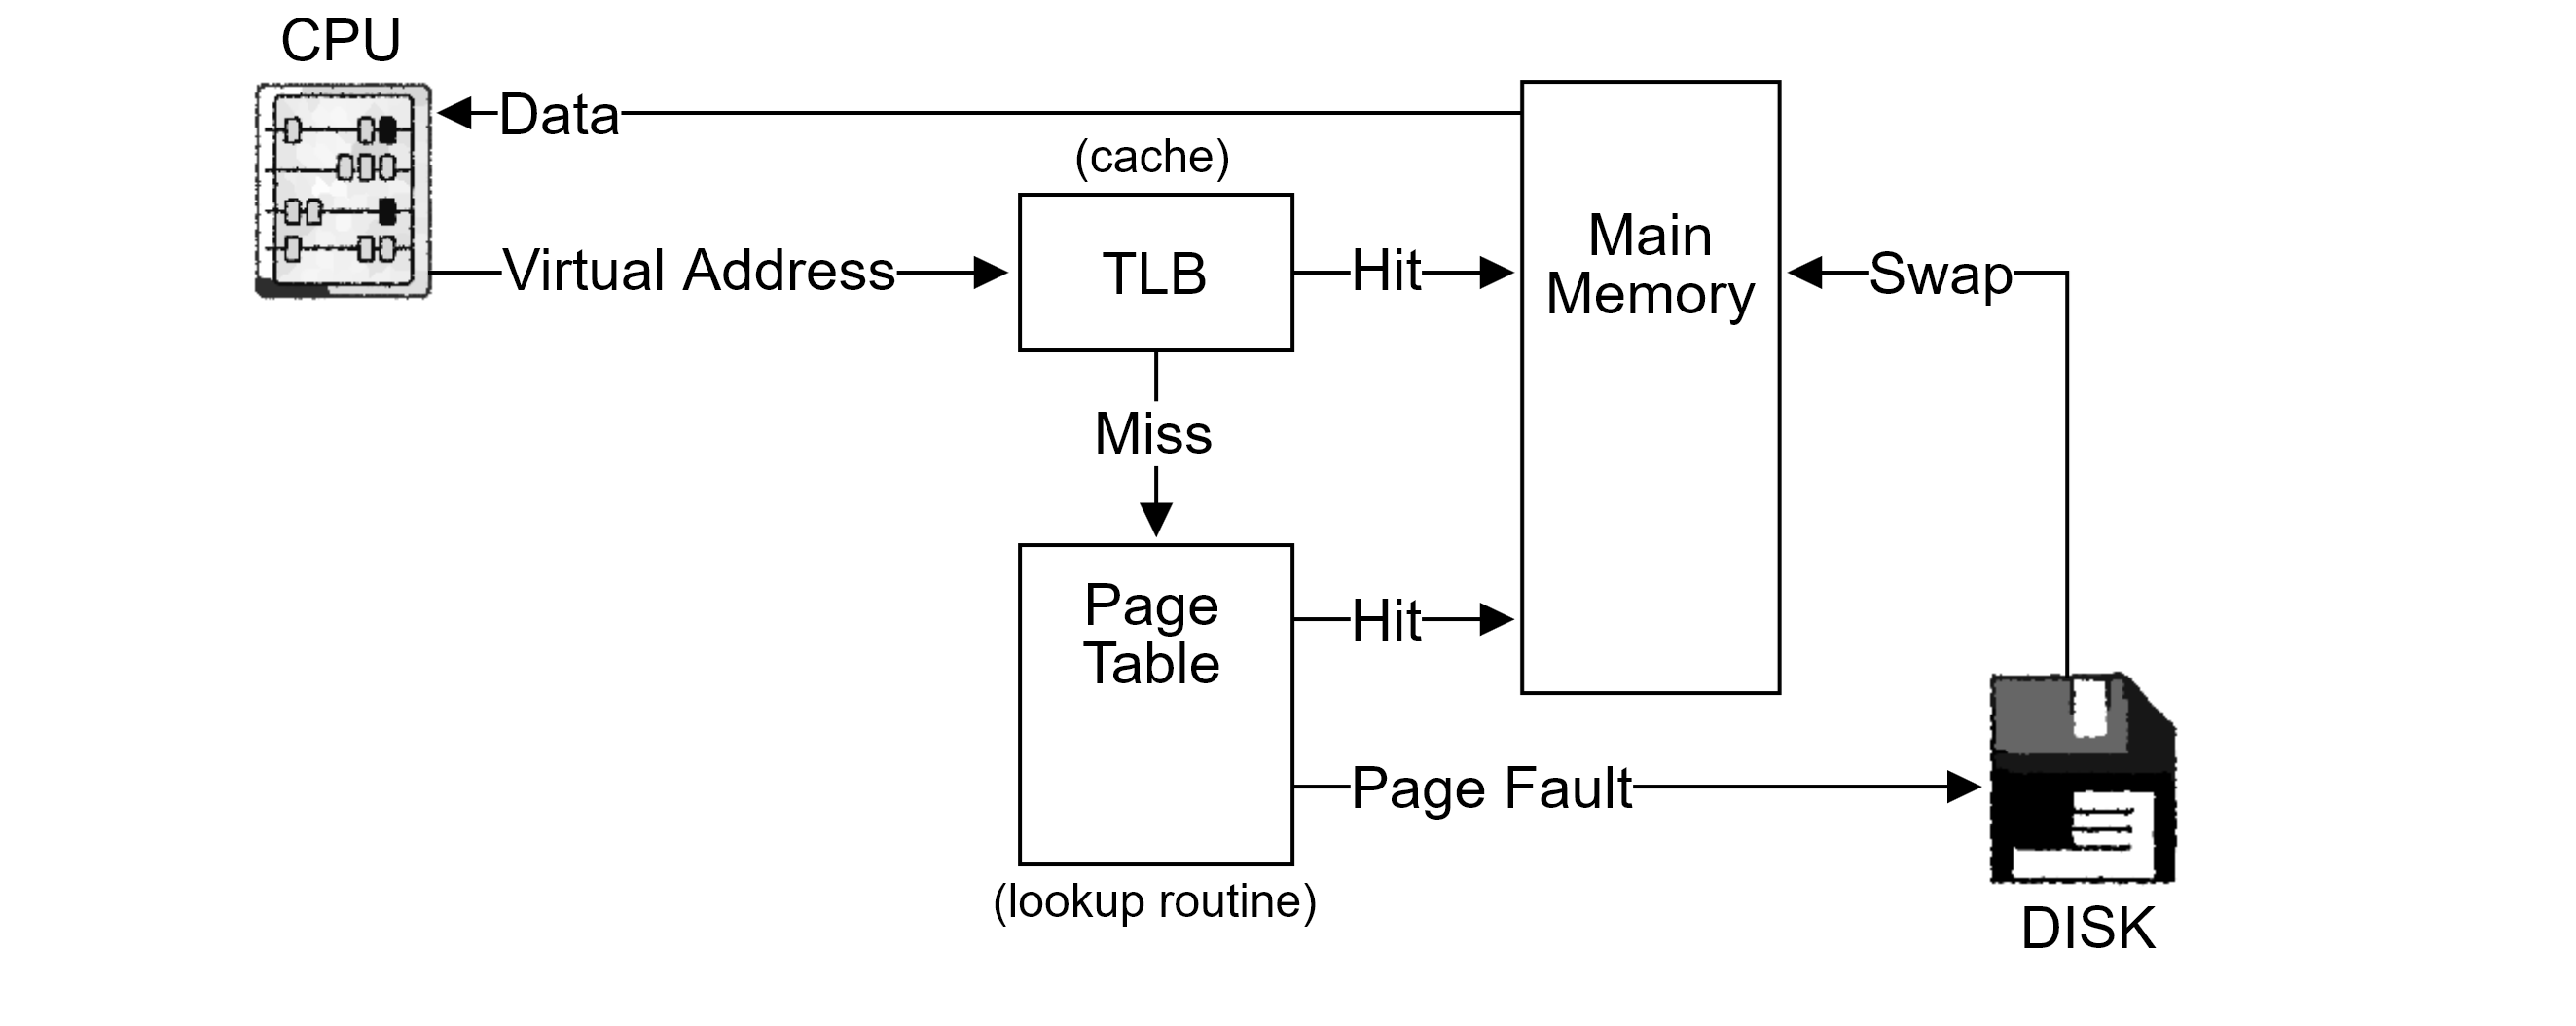
\includegraphics[width=\textwidth]{Sections/virt/tlb.png}
    
    \vspace{1em}
    \caption{Demonstrating how a TLB lookup effects the memory access flow. CPU attempts to access memory providing 
    the virtual address to the TLB. (Happy path) A hit occurs, memory is accessed and passed to the CPU. (Ok path) A TLB miss occurs, causing a page table lookup. A page table hit occurs, the mapping is cached and the memory is accessed. (Sad path) both a TLB and page table miss occurs, causing a page fault. The OS must decide 
    which page to swap out. After swapping, the addressed is cached and the memory is accessed.}
    
    \label{fig:virt7}
\end{figure}

\newpage 
\noindent
So far what we've been covering actually resides within the CPU architecture:
\begin{Def}[Memory Management Unit (MMU)]

    The \textbf{Memory Management Unit (MMU)} is a hardware component that manages the mapping of virtual to physical memory. It is responsible for translating virtual addresses to physical addresses, and it also handles page faults and TLB lookups.
\end{Def}

\subsection{Multi-level Page Tables}

\noindent
Let's define the problem space of multi-level page tables \cite{neso_vm_multilevel}:
\begin{theo}[Single Level Page Table Cost]

    In a 32-bit system, each page table requires 4 MiB of memory. If we had 100 programs running, that's easily 400 MiB of memory.\\

    \noindent
    Additionally, if we move page tables to disk (external storage), we lose any reference we had to them in an attempt to free up memory. So we need to keep some reference oracle in memory.
\end{theo}

\noindent
This highlights the need for a more efficient way 
\begin{Def}[Multi-level Page Tables]

    Recall that in a 32-bit system, we have 4 GiB of memory. In single level page tables, we chunk our addresses into 4 KiBs (4096 bytes), 
    and load all of them at once. That's
    $$4 \text{ KiB} \cdot 1024 \text{ PTEs } = 4096 \text{ KiB} = 4 \text{ MiB }$$

    \noindent
    We wish to offload data without losing references. To do this we allocate a single chunk of memory (4 KiB) to 
    serve as an reference oracle, called the \textbf{page directory} or \textbf{1$^{st}$ level page table}. Each entry in the page directory points to other chunks from which we are safe to load and unload out of memory.
    These referenced chunks are called the \textbf{2$^{nd}$ level page tables}. Each entry in the 2$^{nd}$ level page table points to a physical page.
\end{Def}

\begin{Def}[Converting Virtual to Physical Memory (Multi-level)]

    In multi-level page tables, the first 12 bits are the \textbf{offset}, the next 10 bits are the index into the \textbf{second-level page table}, and the last 10 bits are the index into the \textbf{first-level page directory}. These tables are treated as arrays: indexing the first table yields the address of the second table, and indexing the second table yields the physical page number.
\end{Def}

\newpage 

\noindent
Recall, in single-level page tables the higher 20 bits are the page number and the index, which yields the physical page number.
Multi-level breaks away from this, and instead as illustrated below:
\begin{figure}[h]
    \centering
    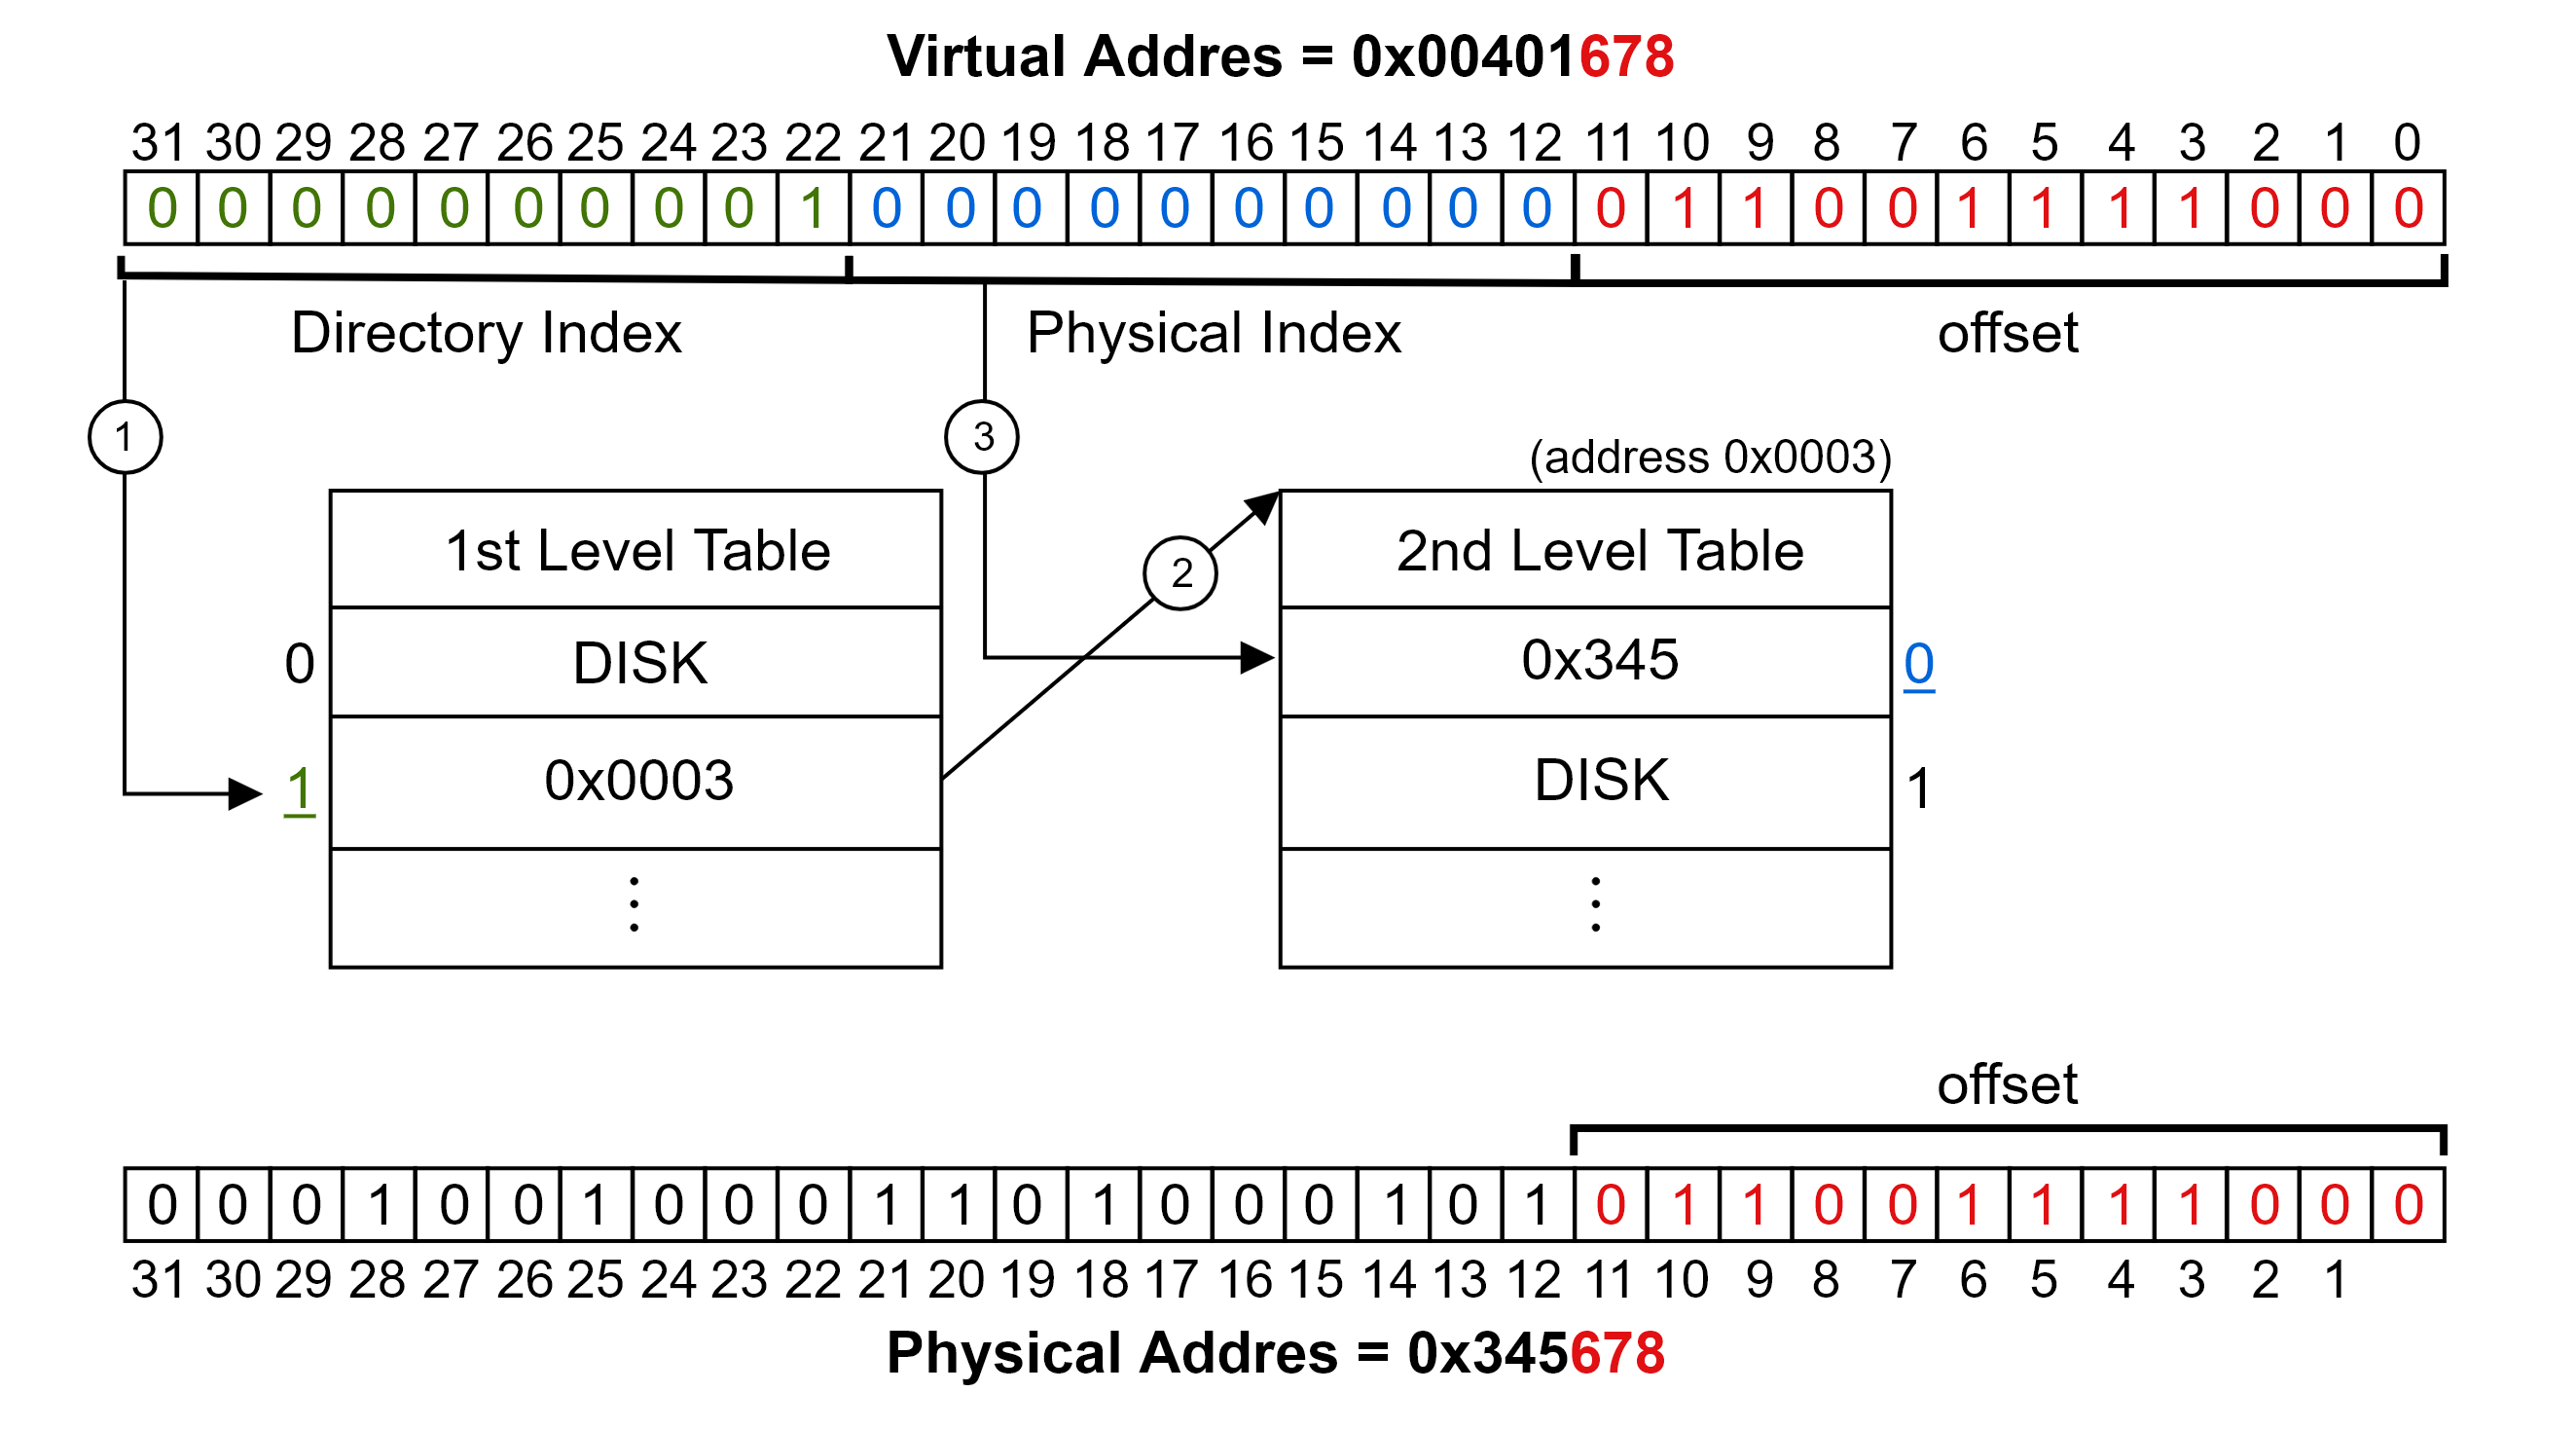
\includegraphics[width=\textwidth]{Sections/virt/level.png}
    
    \vspace{1em}
    \caption{A multi-level page table, where the first level is a page directory, and the second level is a page table which points to physical pages.}
    
    \label{fig:virt8}
\end{figure}

\begin{Def}[Multi-level Page Scaling (64-bit)]

    Increasing the number of bits allows us to scale the number of levels in our page table.
    In 64-bit architectures using 4-level paging (e.g., x86-64), only the lower 48 bits are used. The virtual address is divided into five parts:
    \begin{itemize}
        \item 12 bits for the page offset
        \item 9 bits for the 4$^{\text{th}}$-level page table (PT)
        \item 9 bits for the 3$^{\text{rd}}$-level page directory (PD)
        \item 9 bits for the 2$^{\text{nd}}$-level page directory pointer table (PDPT)
        \item 9 bits for the 1$^{\text{st}}$-level page map level 4 (PML4)
    \end{itemize}
    \noindent
    Modern versions of Windows and Linux support 5 levels, which allows for a maximum of 129 PiB, while 4 gives us 256 TiB.
\end{Def}

\newpage 

\noindent
Finally we talk about the performance of our lookups:

\begin{Def}[Effective Memory Access Time (EMAT)]

    Effective Memory Access Time (EMAT) accounts for the time it takes to access memory in the presence of a Translation Lookaside Buffer (TLB), multi-level paging, and potential page faults.
    Given:
    \begin{itemize}
        \item $t$ = TLB access time;\hspace{3.4em} $m$ = Memory access time
        \item $S$ = Page fault service time;\quad $n$ = Number of page levels
        \item $h$ = TLB hit rate;\hspace{5.1em} $p$ = Page hit rate (1 - page fault rate)
    \end{itemize}

    The EMAT is computed as:

    \[
    \text{EMAT} =
    h(t + m) +
    (1 - h)\left(t + p(n \cdot m) + (1 - p)S\right)
    \]
    \noindent
    Essentially \cite{69017},
    \begin{lstlisting}
        EMAT=
        TLB hit*(TLB access time + Memory access time)
        + TLB Miss*(TLB access time + PageHit*[n * memory access time]
        + PageMiss*PageFaultServiceTime)
    \end{lstlisting}
\end{Def}
\begin{Example}[Three-Level Paging System]

    Suppose the system has:
    \begin{itemize}
        \item $n = 3$ page levels
        \item $t = 5$ ns (TLB lookup)
        \item $m = 100$ ns (memory access time)
        \item $\alpha = 0.80$ (TLB hit rate)
    \end{itemize}

    \noindent
    Then the EMAT is:
    \begin{align*}
    \text{EMAT} &=
    (5 + 100)\cdot 0.80 +
    (5 + 3 \cdot 100 + 100)\cdot (1 - 0.80)\\
    &= 105 \cdot 0.80 + 405 \cdot 0.20 = 84 + 81 = \boxed{165\ \text{ns}}
    \end{align*}

    \noindent
    For a better TLB hit rate $\alpha = 0.98$:
    
    \vspace{-1em}
    \begin{align*}
        \hspace{4.3em}\text{EMAT} =
        105 \cdot 0.98 + 405 \cdot 0.02 = 102.9 + 8.1 = \boxed{111\ \text{ns}}  && \cite{amir2003multilevel}
    \end{align*}
\end{Example}

